\section{Dispersion and directional filtering}
\label{sec:results}

The results separate two mechanisms: Case~H isolates the effect of an oriented characteristic-length tensor in a homogeneous medium, whereas Case~C adds periodic material contrast. The first controls direction-dependent dispersion and steering; the second can open a complete gap, although its reported width is mesh-sensitive. Selected inputs are summarized in Table~\ref{tab:case_params}; the extended parameter set is given in Supplementary Material~S1.

\begin{table}[htbp]
\centering
\caption{Selected material and numerical inputs for Cases H and C and the steering analysis.}
\label{tab:case_params}
\begin{tabularx}{\textwidth}{@{}l p{3.0cm} Y@{}}
\toprule
Case & Quantity & Value \\
\midrule
H & Cell and matrix & $L=1.0\,\mathrm{m}$; $\lambda=\mu=1.0\,\mathrm{Pa}$; $\rho=1.0\,\mathrm{kg/m^3}$ \\
H & Lengths and mesh & $l_{\mathrm{iso}}=0.20\,\mathrm{m}$; $\ell_{\mathrm{i}}=0.20\,\mathrm{m}$; $16\times16$ BFS elements per cell \\
C & Epoxy matrix & $\rho_m=1142\,\mathrm{kg/m^3}$; $\mu_m=1.48\,\mathrm{GPa}$; $\lambda_m=4.57\,\mathrm{GPa}$ \\
C & YBCO inclusion & $\rho_i=6333\,\mathrm{kg/m^3}$; $\mu_i=37.0\,\mathrm{GPa}$; $\lambda_i=95.0\,\mathrm{GPa}$ \\
C & Geometry and length scales & $L=1.0\,\mathrm{m}$; $r_0/L=0.30$; $\ell_m/L=0.10$; $\ell_i/L=0.20$ \\
C & Frequency scale and reported resolution & $c_{t,m}=1138.4\,\mathrm{m/s}$; $\omega_{0,C}=\pi c_{t,m}/L=3576.4\,\mathrm{rad/s}$; $4\times4$ mesh and $21\times21$ zone grid \\
Steering & Acoustic-branch sweep & $\bar{k}=0.5$; $\mathrm{AR}\in\{5,10\}$; $\theta=0^\circ,15^\circ,\ldots,90^\circ$ \\
\bottomrule
\end{tabularx}

\end{table}

\subsection{Anisotropy reshapes the homogeneous spectrum}
Figure~\ref{fig:caseH_dispersion} compares the isotropic reference with two orientations of the anisotropic length tensor. Both acoustic branches emerge from zero frequency at $\Gamma$, while changes in aspect ratio and orientation shift the branches and lift symmetry-related degeneracies at the zone edge. For $\mathrm{AR}=10$ and $\theta=45^\circ$, a narrow stop band opens along $\Gamma$--$X$, with $\Delta_{GX}=0.0043$. It is directional rather than complete: modes on other propagation directions overlap this interval, and the full-zone complete-gap measure remains $\Delta_{\mathrm{complete}}\le -0.3235$.

\begin{figure}[htbp]
\centering
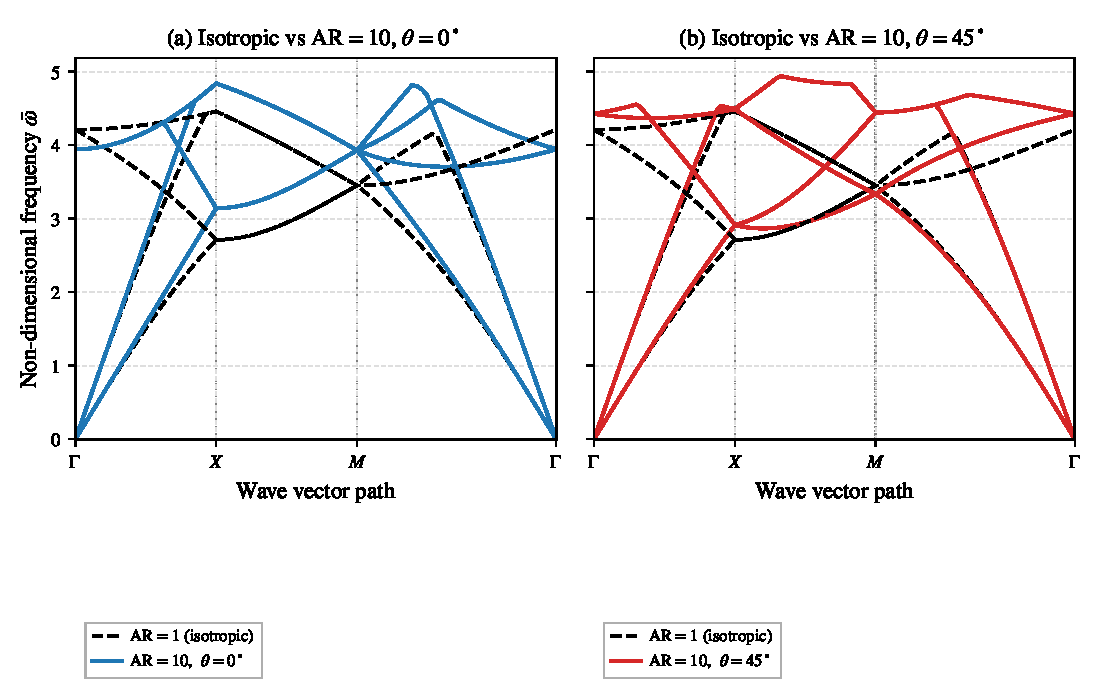
\includegraphics[width=\textwidth]{figures/fig06_caseH_dispersion.pdf}
\caption{Case-H Bloch bands along $\Gamma$--$X$--$M$--$\Gamma$. (a) Isotropic reference ($\mathrm{AR}=1$) and aligned anisotropy ($\mathrm{AR}=10$, $\theta=0^\circ$). (b) Isotropic reference and diagonal anisotropy ($\mathrm{AR}=10$, $\theta=45^\circ$), which opens a $\Gamma$--$X$ stop band but no complete gap.}
\label{fig:caseH_dispersion}
\end{figure}

The orientation sweep in Figure~\ref{fig:theta_sweep} shows how rotation redistributes the zone-edge frequencies. At $\mathrm{AR}=5$, as $\theta$ changes from $0^\circ$ to $90^\circ$, the transverse and longitudinal frequencies at $X$ decrease from $2.915$ to $2.672$ and from $5.050$ to $4.628$, respectively, as the projected length scale changes from the major to the minor axis. The $M$-point frequencies exhibit reflection symmetry about $45^\circ$, consistent with the square-cell symmetry.

\begin{figure}[htbp]
\centering
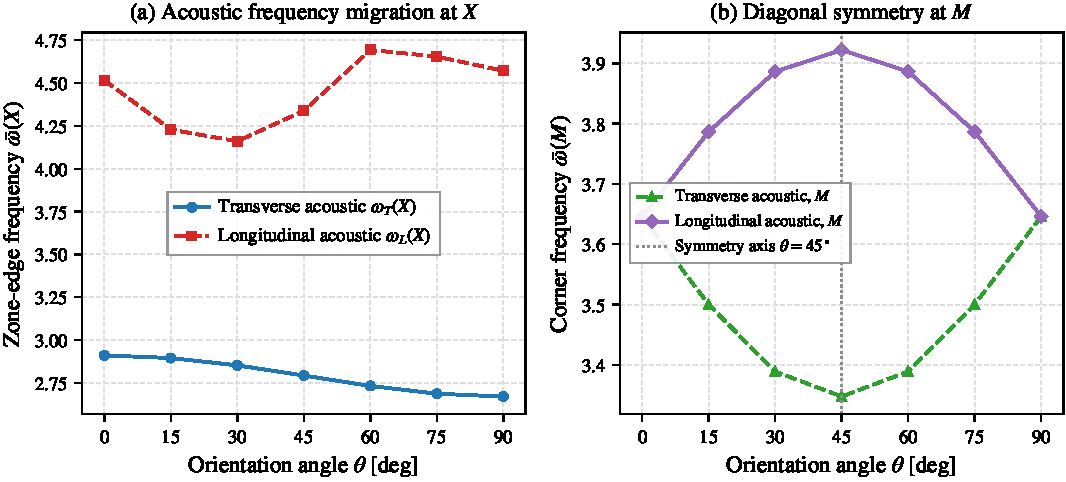
\includegraphics[width=\textwidth]{figures/fig08_theta_sweep.pdf}
\caption{Orientation dependence of the first four Case-H eigenfrequencies at (a) $X$ and (b) $M$ for $\mathrm{AR}=5$. The $M$-point response is symmetric about $\theta=45^\circ$.}
\label{fig:theta_sweep}
\end{figure}

Figure~\ref{fig:ar_sweep} isolates the effect of elongation at $\theta=45^\circ$. The isotropic case already has an orientation-independent directional width $\Delta_{GX}=0.041$; increasing $\mathrm{AR}$ changes the relative branch positions, but the directional gap is not monotone in aspect ratio.

\begin{figure}[htbp]
\centering
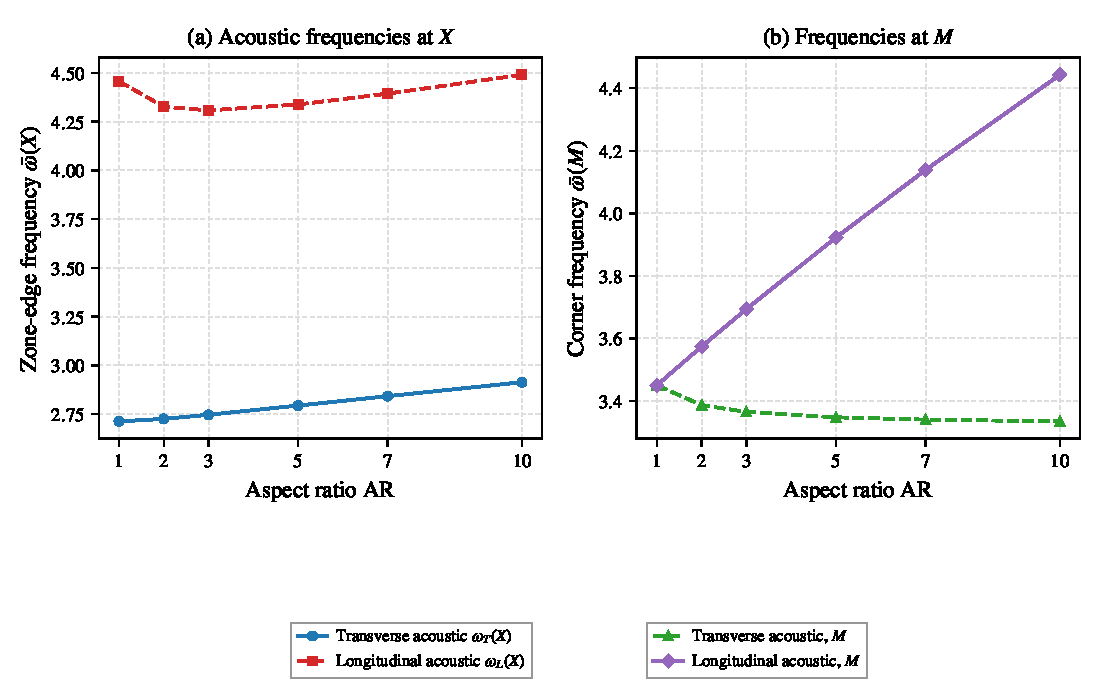
\includegraphics[width=\textwidth]{figures/fig09_ar_sweep.pdf}
\caption{Case-H branch frequencies at $X$ and $M$ as the aspect ratio varies from $1$ to $10$ at fixed $\theta=45^\circ$, using volume-equivalent length scaling.}
\label{fig:ar_sweep}
\end{figure}

The combined $(\theta,\mathrm{AR})$ sample in Figure~\ref{fig:design_map} identifies a maximum $\Delta_{GX}=0.0677$ at $(0^\circ,7)$ among 42 evaluated configurations; the response is non-monotone in aspect ratio. The plotted surface interpolates these evaluated points and is not a continuous optimization. The polar view in Figure~\ref{fig:polar_map} recasts the same sampled values by the sign of $\Delta_{GX}$; its regime boundary is descriptive of the sampled response.

\begin{figure}[htbp]
\centering
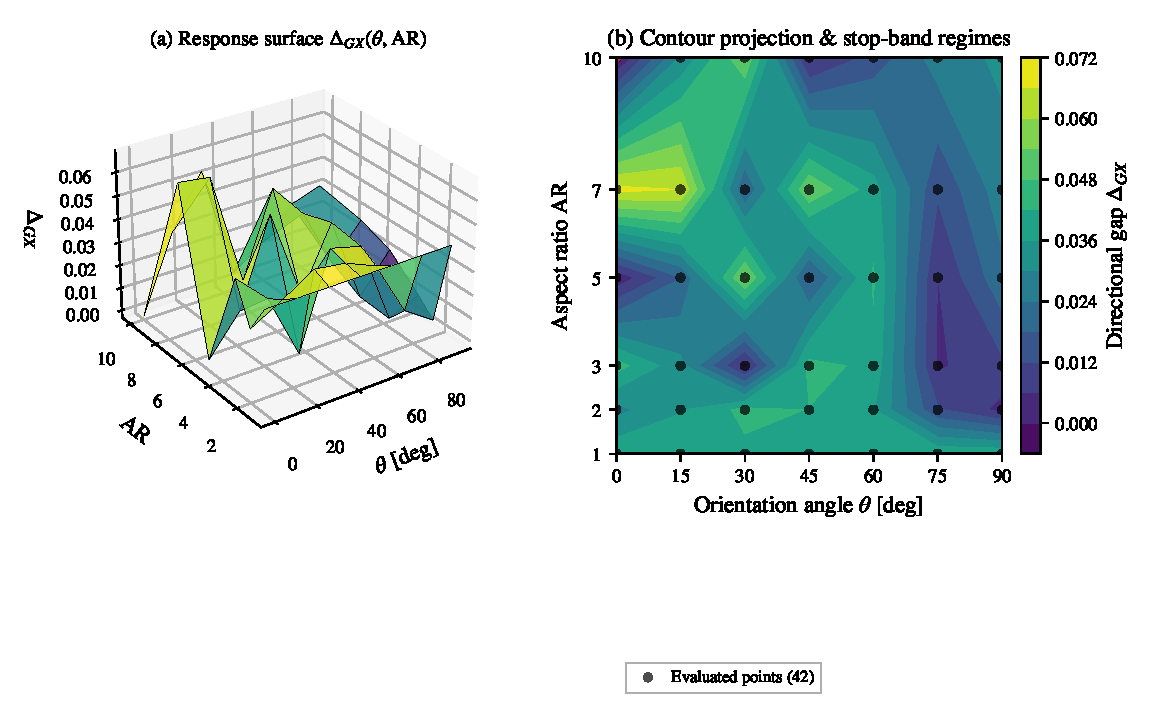
\includegraphics[width=\textwidth]{figures/fig10_design_map_3d.pdf}
\caption{Sampled Case-H design response $\Delta_{GX}(\theta,\mathrm{AR})$ for 42 configurations. The largest sampled value is $0.0677$ at $\theta=0^\circ$, $\mathrm{AR}=7$; at $\theta=45^\circ$, $\mathrm{AR}=10$, $\Delta_{GX}=0.0043$.}
\label{fig:design_map}
\end{figure}

\begin{figure}[htbp]
\centering
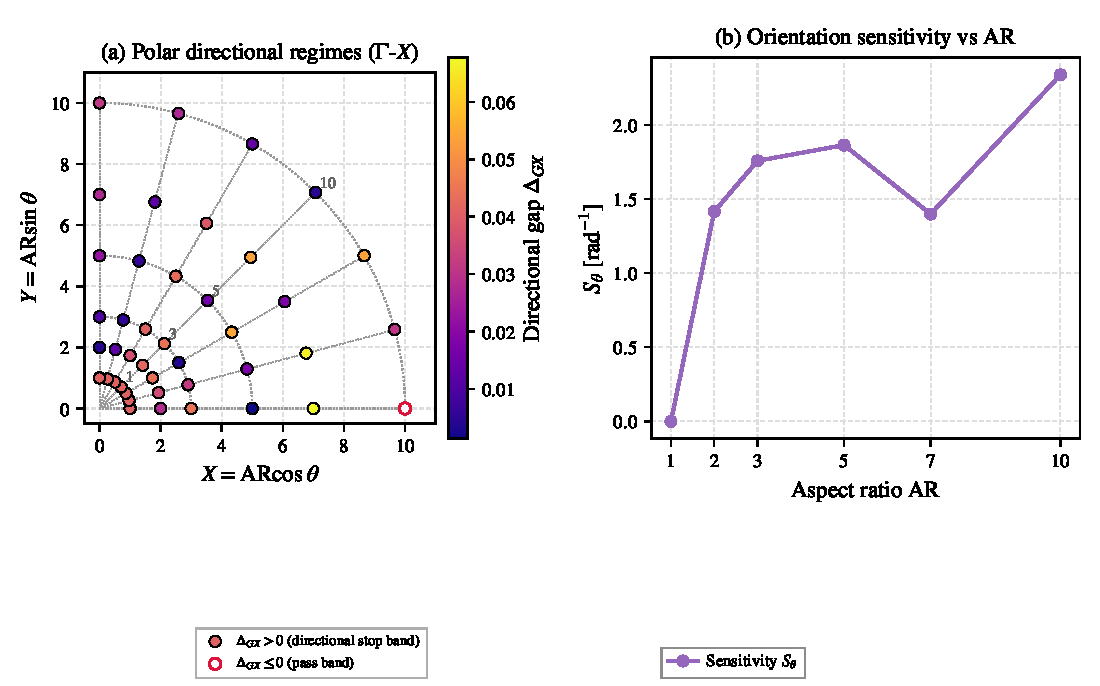
\includegraphics[width=\textwidth]{figures/fig11_polar_map_regimes.pdf}
\caption{Polar-coordinate view of the sampled Case-H designs, classified by $\Delta_{GX}\le0$ (pass band) and $\Delta_{GX}>0$ (directional stop band). The displayed boundary is a visual summary of sampled points.}
\label{fig:polar_map}
\end{figure}

Table~\ref{tab:gap_summary} summarizes representative directional and complete-gap measures. The complete-gap values remain negative for every listed homogeneous configuration, while the orientation sensitivity $S_\theta$ is largest at $\mathrm{AR}=10$ ($2.34\,\mathrm{rad}^{-1}$). The normalized widths and mesh-to-mesh variations are reported in Supplementary Material~S3.

\begin{table}[htbp]
\centering
\caption{Directional and complete-gap measures for representative Case-H configurations; values are reported at the precision retained between the $8\times8$ and $16\times16$ meshes.}
\label{tab:gap_summary}
\begin{tabularx}{\textwidth}{@{}c c r r r@{}}
\toprule
$\mathrm{AR}$ & $\theta$ & $\Delta_{GX}$ & $\Delta_{\mathrm{path}}$ & $\Delta_{\mathrm{complete}}$ \\
\midrule
$1$ & $0^\circ$  & $+0.041$ & $-0.32$ & $-0.32$ \\
$1$ & $45^\circ$ & $+0.041$ & $-0.32$ & $-0.32$ \\
$1$ & $90^\circ$ & $+0.041$ & $-0.32$ & $-0.32$ \\
$3$ & $0^\circ$  & $+0.045$ & $-0.10$ & $-0.46$ \\
$3$ & $45^\circ$ & $+0.044$ & $-0.45$ & $-0.48$ \\
$3$ & $90^\circ$ & $+0.011$ & $-0.33$ & $-0.46$ \\
$5$ & $0^\circ$  & $+0.001$ & $-0.01$ & $-0.58$ \\
$5$ & $45^\circ$ & $+0.016$ & $-0.48$ & $-0.58$ \\
$5$ & $90^\circ$ & $+0.022$ & $-0.37$ & $-0.58$ \\
$10$ & $0^\circ$  & $-0.002$ & $-0.24$ & $-0.85$ \\
$10$ & $45^\circ$ & $+0.004$ & $-0.29$ & $-0.56$ \\
$10$ & $90^\circ$ & $+0.031$ & $-0.65$ & $-0.85$ \\
\midrule
\multicolumn{5}{@{}l@{}}{$S_\theta$ [rad$^{-1}$]: AR $=1$: $0.00$; $2$: $1.42$; $3$: $1.76$; $5$: $1.86$; $7$: $1.40$; $10$: $2.34$.} \\
\bottomrule
\end{tabularx}

\end{table}

\subsection{Periodic material contrast opens a complete gap}
\label{sec:caseC_pc}
Unlike homogeneous Case~H, Case~C combines gradient elasticity with a periodic epoxy--YBCO impedance contrast ($\chi_\mu=25.0$, $\chi_\rho=5.546$; Table~\ref{tab:case_params}). The cell period is denoted $L$ here and $a$ in Figure~\ref{fig:caseC_dispersion}; $r_0/L=r_0/a=0.30$ gives a filling fraction of $28.27\%$. Figure~\ref{fig:caseC_dispersion} shows a complete gap between Bands~3 and~4 over $\bar{\omega}\in[4.5698,7.1430]$, giving $\Delta_{\mathrm{complete}}=2.5732$ or $43.94\%$ on the $4\times4$ mesh and $21\times21$ Brillouin-zone grid. The circular interface is integrated by sub-cell Gauss sampling on the Cartesian mesh. Brillouin-zone refinement changes the quoted width by less than $4\times10^{-4}$, but finite-element refinement has a much larger effect.

\begin{figure}[htbp]
\centering
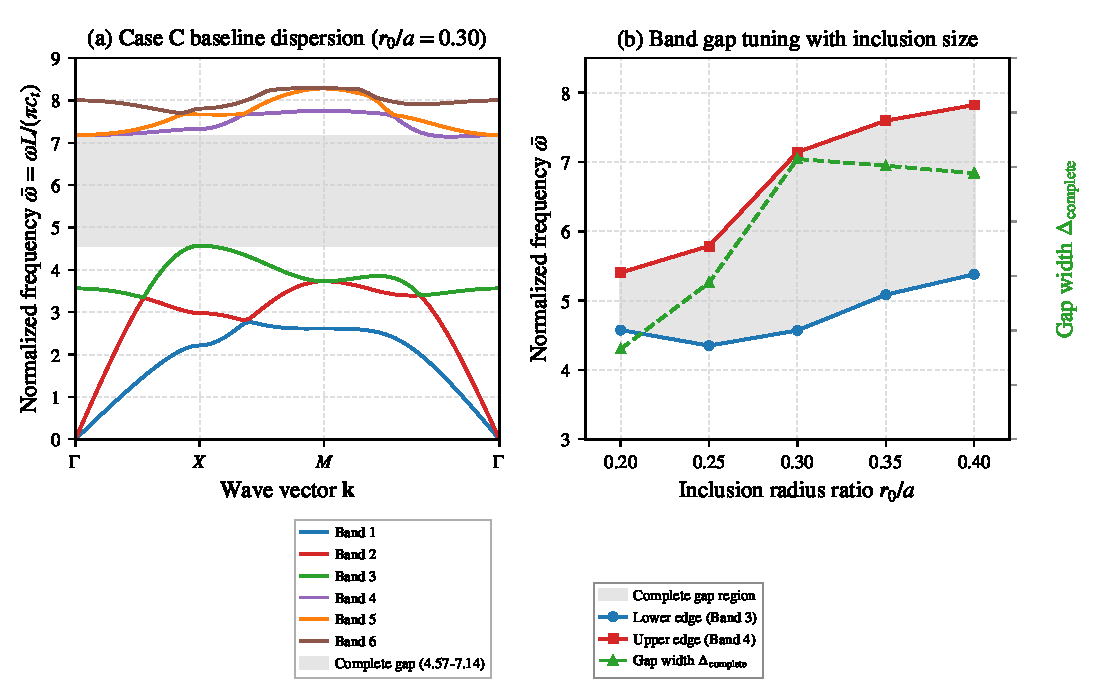
\includegraphics[width=\textwidth]{figures/fig07_caseC_dispersion.pdf}
\caption{Case-C complete-gap formation and radius dependence. (a) Bands along $\Gamma$--$X$--$M$--$\Gamma$ for $r_0/L=0.30$, with the $4\times4$-mesh gap between Bands~3 and~4. (b) Complete-gap width versus $r_0/a$ at the same mesh; the $r_0/a=0.30$ result is not mesh-converged.}
\label{fig:caseC_dispersion}
\end{figure}

The complete gap decreases monotonically from $2.5732$ at $4\times4$ to $2.2504$, $2.0722$, $1.9736$, and $1.9179$ at $8\times8$, $16\times16$, $32\times32$, and $64\times64$, respectively. It remains open at each computed resolution but is not mesh-converged; $2.5732$ is therefore a coarse-mesh result, not a converged continuum value. At the $4\times4$ mesh, increasing $r_0/L$ from $0.20$ to $0.30$ widens the gap from $0.8288$ ($16.61\%$) to $2.5732$ ($43.94\%$), after which it narrows to $2.4426$ ($37.00\%$) at $r_0/L=0.40$. Additional mesh, quadrature, and zone-sampling details are provided in Supplementary Material~S4.
